%& preamble - kommer användas i subfiles med
\documentclass{article}
\usepackage[utf8]{inputenc}
\usepackage{parskip}
\usepackage{pgffor}
\usepackage{amsmath}
\usepackage{tikz}
\usepackage{tkz-euclide}
\usepackage{pdfpages}

% lägg till egna macros
% för att enkelt formattera lösningar
\newenvironment{solution}[1]
    {\addcontentsline{toc}{subsubsection}{#1}{\Large\textbf{#1.}}\newline}
    {\newline}

\newcommand{\subsolution}[1]{{\large\textbf{#1)}\newline}}

% för att skapa "formler"
\newtheorem{formel}{Formel}

% kommando för att skriva R^n
\newcommand{\Rn}[1]{\mathbb{R}^{#1}}

% environment för att enkelt skapa rutnät där man kan rita vektorer
\newenvironment{vectors2d}[4]
{
\begin{center}
\begin{tikzpicture}[scale=0.5]
  \draw[thin,gray!40] (#1,#2) grid (#3,#4);
  \draw[<->] (#1,0)--(#3,0) node[right]{$x$};
  \draw[<->] (0,#2)--(0,#4) node[above]{$y$};
}
{
\end{tikzpicture}
\end{center}
}
% Lägg in sånna här för att rita vektorer:
% \draw[line width=1pt,gray!40,-stealth](2,3)--(1,-2) node[anchor=south west]{$\vec{u}$};
% om man vill färga den:
% \draw[line width=1pt,blue,-stealth](2,3)--(1,-2) node[anchor=south west]{$\vec{u}$};


%% inkludera alla lösningar i en mapp 
%% uppgifter som saknas skrivs upp i table of contents med, fast som missing
\newcommand{\inkluderauppgifter}[2]{
\foreach \i in {1, ..., #2} {
    \edef\FileName{#1/\i}%
    \IfFileExists{\FileName}{%
       \subfile{\FileName}%
    }{%else
        {\addcontentsline{toc}{subsubsection}{\color{red} \i - lösning saknas}}%
    }%
}%
}




%% totalmatris
% https://tex.stackexchange.com/questions/2233/whats-the-best-way-make-an-augmented-coefficient-matrix
\makeatletter
\renewcommand*\env@matrix[1][*\c@MaxMatrixCols c]{%
  \hskip -\arraycolsep
  \let\@ifnextchar\new@ifnextchar
  \array{#1}}
\makeatother

\usepackage{subfiles} % inkluderar allt innan i subfiles, så bör komma sist.


\title{SF1624 - Algebra och geometri\\ {\large detaljerade lösningar till rekommenderade uppgifter för modul 1}}
\author{Simon Rosén, Harald Olin}
\date{October 2022}

\begin{document}

%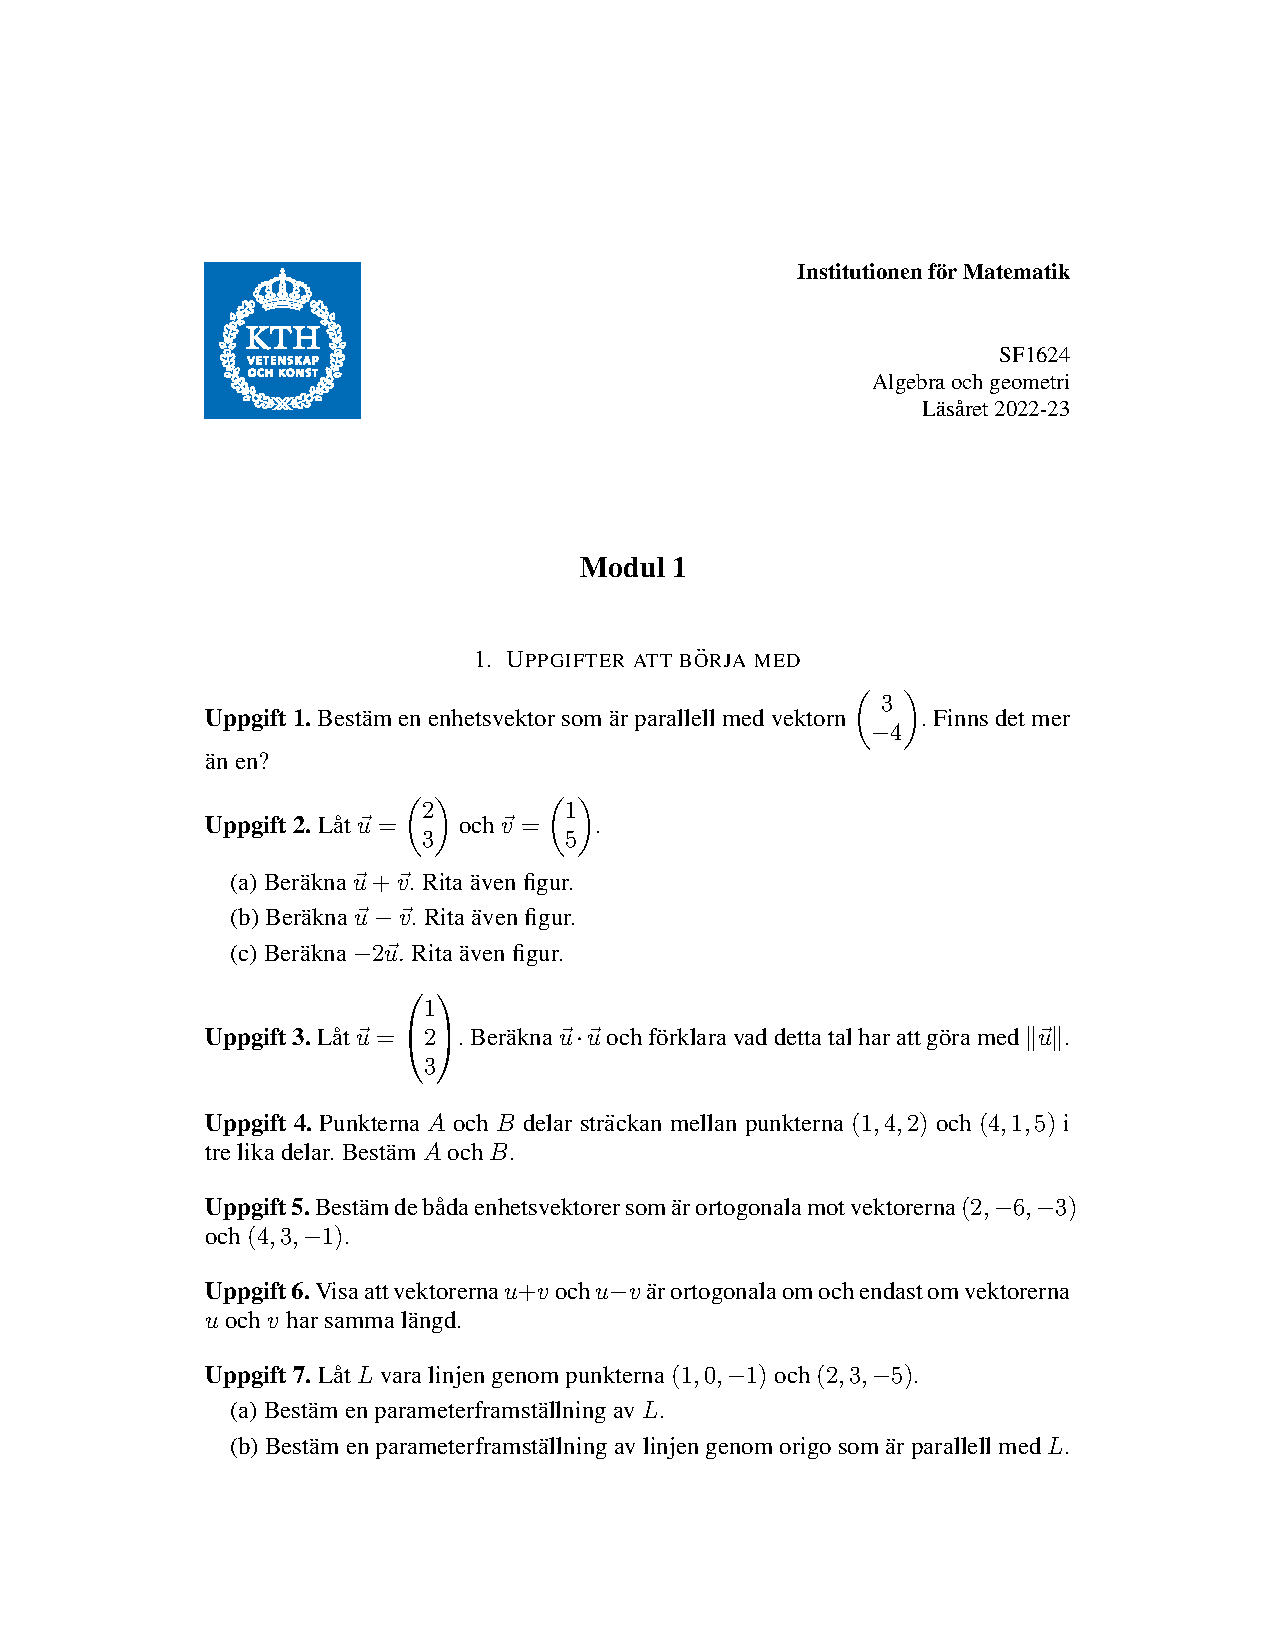
\includepdf[pages=-]{pdfs/22Modul1.pdf} % ska nog inte vara med i slutgiltig version, men nice att ha när man löser uppgifterna

\maketitle
\section{Teori}

Vektorerna i dessa exempel är tre dimensioner ($\Rn{3}$). Men formlerna fungerar på liknande sätt för en godtycklig dimension ($\Rn{n}$).

\begin{formel}{(vektoraddition)}\\
\label{vecadd}
Två vektorer $\vec{u} = (u_1, u_2, u_3)$ och $\vec{v} = (v_1, v_2, v_3)$ adderas såhär:
\[
\vec{u} + \vec{v} = (u_1 + v_1, u_2 + v_2, u_3 + v_3)
\]

Kom ihåg att $\vec{u} - \vec{v} = \vec{u} + (-1)\cdot\vec{v}$
\end{formel}

\begin{formel}{(vektormultiplikation med ett tal)}\\
\label{vecscale}
Ett tal $t$ och en vektor $\vec{u} = (u_1, u_2, u_3)$ multipliceras såhär:
\[
t \cdot \vec{u} = (t \cdot u_1, t \cdot u_2, t \cdot u_3)
\]
\end{formel}


\begin{formel}
\label{veclength}
Längden $|\vec{v}|$ av en vektor $\vec{v} = (x, y, z)$ fås genom:
\[
|\vec{v}| = \sqrt{x^2+y^2+z^2}
\]

\end{formel}

\begin{formel}
\label{unitvec}
En enhetsvektor $\vec{e}_\vec{v}$ i samma riktning som en vektor $\vec{v}$ fås genom:
\[
    \vec{e}_{\vec{v}} = \frac{1}{|\vec{v}|} \cdot \vec{v} 
\]

Man skalar alltså om vektorn så att den får längd ett.
\end{formel}

\begin{formel}{(skalärprodukt)}
\label{skalarprod}
Skalärprodukten av två vektorer $\vec{u} = (u_1, u_2, u_3)$ och $\vec{v} = (v_1, v_2, v_3)$ är:
\[
\vec{u} \cdot \vec{v} = u_1 \cdot v_1 + u_2 \cdot v_2 + u_3 \cdot v_3
\]

En annan formel som kan användas är: 
\[
\vec{u} \cdot \vec{v} = |\vec{u}||\vec{v}|sin(\alpha)
\]
Där $\alpha$ är vinkeln mellan vektorerna $\vec{u}$ och $\vec{v}$. Denna formel är särskilt användbar om man vill räkna ut vinkeln mellan två vektorer.

Skalärprodukten av två vektorer är ett tal.
\end{formel}

\begin{formel}{(krysspordukt)}
\label{kryssprod} 
Kryssprodukten av två vektorer $\vec{u} = (u_1, u_2, u_3)$ och $\vec{v} = (v_1, v_2, v_3)$ är
\[\vec{u}\times \vec{v} = (u_2\cdot v_3 - u_3\cdot v_2, u_2\cdot v_3 - u_3\cdot v_2, u_2\cdot v_3 - u_3\cdot v_2)\]

En annan formel som kan användas för att beräkna kryssprodukten är
\[\vec{u}\times \vec{v} = |\vec{u}||\vec{v}|sin(\alpha)\]
Där $\alpha$ är vinkeln mellan $\vec{u}$ och $\vec{v}$.

En viktig egenskap kryssprodukten $\vec{u}\times\vec{v}$ är att den är en vektor som är ortogonal mot båda vektorerna $\vec{u}$ och $\vec{v}$.
\end{formel}

\section{Uppgifter}

% include på alla uppgifter
\foreach \i in {1, ..., 99} {
    \edef\FileName{uppgifter/\i}%
    \IfFileExists{\FileName}{%
       \subfile{\FileName}%
    }
}

\end{document}
